% arara: xelatex
%% arara: xelatex


% https://koalatea.io/r-knn-regression/
% http://freerangestats.info/blog/2017/04/09/propensity-v-regression
% https://economics.stackexchange.com/questions/45335/what-is-the-difference-between-ate-and-att
% https://kosukeimai.github.io/MatchIt/articles/matching-methods.html


\documentclass[14pt,xcolor=dvipsnames]{beamer}


% !TEX root = om_metrics_14.tex

%\usepackage{epsdice} % dice 1-6 for probability :)

% \usepackage[absolute,overlay]{textpos}

% \usefonttheme[onlymath]{serif}

\usefonttheme{professionalfonts}
% by default beamer changes math fonts for better visibility for projection
% this professionalfonst theme removes this behavior


\usepackage[orientation=portrait,size=custom,width=25.4,height=19.05]{beamerposter}




%25,4 см 19,05 см размеры слайда в powerpoint

\usetheme{metropolis}
\metroset{
  %progressbar=none,
  numbering=none,
  subsectionpage=progressbar,
  block=fill
}

%\usecolortheme{seahorse}

\usepackage{xunicode} % хак для акцентов!
% https://tex.stackexchange.com/questions/28003/

\usepackage{fontspec}
\usepackage{polyglossia}
\setmainlanguage{russian}


% \usepackage{fontawesome5} % removed [fixed]
\setmainfont[Ligatures=TeX]{Myriad Pro}
% \setsansfont{Myriad Pro}




% why do we need \newfontfamily:
% http://tex.stackexchange.com/questions/91507/
\newfontfamily{\cyrillicfonttt}{Myriad Pro}
\newfontfamily{\cyrillicfont}{Myriad Pro}
%\newfontfamily{\cyrillicfontbs}{Myriad Pro}
\newfontfamily{\cyrillicfontsf}{Myriad Pro}


% https://tex.stackexchange.com/questions/175860/why-does-unicode-math-break-the-kerning-of-accents-in-combination-with-amssymb
% "You shouldn't be using amssymb together with unicode-math"
\usepackage{amsmath}
\usepackage{amsthm} % amssymb 


% https://tex.stackexchange.com/questions/483722/
% \usepackage[MnSymbol]{mathspec}  % Includes amsmath.
% \usepackage{mathspec}  % Includes amsmath.
% \setmathsfont(Digits,Latin,Greek,Symbols)[Numbers={Lining,Proportional}]{Latin Modern Math}
% mathspec must be loaded earlier than amsmath



%\usepackage{bm}

% \usepackage{fdsymbol} % \nperp

% \usepackage{unicode-math} % \symbf
% \setmathfont{Latin Modern Math}



\usepackage{centernot}

\usepackage{graphicx}

\usepackage{wrapfig}
% \usepackage{animate} % animations :)
% \usepackage{tikz}
%\usetikzlibrary{shapes.geometric,patterns,positioning,matrix,calc,arrows,shapes,fit,decorations,decorations.pathmorphing}
% \usepackage{pifont}
\usepackage{comment}
\usepackage[font=small,labelfont=bf]{caption}
\captionsetup[figure]{labelformat=empty}
% \includecomment{techno}



%Расположение

\setbeamersize{text margin left=15 mm,text margin right=5mm} 
\setlength{\leftmargini}{38 pt}

%\usepackage{showframe}
%\usepackage{enumitem}
% \setlist{leftmargin=5.5mm}


%Цвета от дирекции

\definecolor{dirblack}{RGB}{58, 58, 58}
\definecolor{dirwhite}{RGB}{245, 245, 245}
\definecolor{dirred}{RGB}{149, 55, 53}
\definecolor{dirblue}{RGB}{0, 90, 171}
\definecolor{dirorange}{RGB}{235, 143, 76}
\definecolor{dirlightblue}{RGB}{75, 172, 198}
\definecolor{dirgreen}{RGB}{155, 187, 89}
\definecolor{dircomment}{RGB}{128, 100, 162}

\setbeamercolor{title separator}{bg=dirlightblue!50, fg=dirblue}

%Цвета блоков

% Голубой блок!
\setbeamercolor{block title}{bg=dirblue!30,fg=dirblack}
\setbeamercolor{block title example}{bg=dirlightblue!50,fg=dirblack}
\setbeamercolor{block body example}{bg=dirlightblue!20,fg=dirblack}

\AtBeginEnvironment{exampleblock}{\setbeamercolor{itemize item}{fg=dirblack}}
%\setbeamertemplate{blocks}[rounded][shadow]

% Набор команд для удобства верстки

% Набор команд для структуризации

%\newcommand{\quest}{\faQuestionCircleO}
%\faPencilSquareO \faPuzzlePiece \faQuestionCircleO  \faIcon*[regular]{file} {\textcolor{dirblue}
%\newcommand{\quest}{\textcolor{dirblue}{\boxed{\textbf{?}}}
%\newcommand{\task}{\faIcon{tasks}}
%\newcommand{\exmpl}{\faPuzzlePiece}
%\newcommand{\dfn}{\faIcon{pen-square}}
%\newcommand{\quest}{\textcolor{dirblue}{\faQuestionCircle[regular]}}
%\newcommand{\acc}[1]{\textcolor{dirred}{#1}}
%\newcommand{\accm}[1]{\textcolor{dirred}{#1}}
%\newcommand{\acct}[1]{\textcolor{dirblue}{#1}}
%\newcommand{\acctm}[1]{\textcolor{dirblue}{#1}}
%\newcommand{\accex}[1]{\textcolor{dirblack}{\bf #1}}
%\newcommand{\accexm}[1]{\textcolor{dirblack}{ \mathbf{#1}}}
%\newcommand{\acclp}[1]{\textcolor{dirorange}{\it #1}}
\newcommand{\todo}[1]{\textcolor{dircomment}{\bf #1}}
%\newcommand{\graylink}[1]{{\fontsize{11}{12}\selectfont \textcolor{gray}{#1}}}
%\newcommand{\figcaption}[1]{{\fontsize{18}{20}\selectfont #1}}


\newcommand{\videotitle}[1]{
    {\fontsize{33}{30}\selectfont \textcolor{dirblue}{\textbf{#1}} }

    %\todo{название видеофрагмента}
}

\newcommand{\lecturetitle}[1]{
  {\fontsize{33}{30}\selectfont \textcolor{dirblue}{\textbf{#1}} }

    %\todo{название лекции}
}





%\newcommand{\spcbig}{\vspace{-10 pt}}
%\newcommand{\spcsmall}{\vspace{-5 pt}}

%\usepackage{listings}
%\lstset{
%xleftmargin=0 pt,
%  basicstyle=\small, 
%  language=Python,
  %tabsize = 2,
%  backgroundcolor=\color{mc!20!white}
%}



%\newcommand{\mypart}[1]{\begin{frame}[standout]{\huge #1}\end{frame}}

\setbeamercolor{background canvas}{bg=}

% frame title setup
\setbeamercolor{frametitle}{bg=,fg=dirblue}
\setbeamertemplate{frametitle}[default][left]

\addtobeamertemplate{frametitle}{\hspace*{0.1 cm}}{\vspace*{0.25cm}}


%Шрифты
\setbeamerfont{frametitle}{family=\rmfamily,series=\bfseries,size={\fontsize{33}{30}}}
\setbeamerfont{framesubtitle}{family=\rmfamily,series=\bfseries,size={\fontsize{26}{20}}}


% удобнее знать номер слайда, чтобы вносить правки!  

\setbeamercolor{footline}{fg=dircomment}
\setbeamerfont{footline}{series=\bfseries, size={\fontsize{12}{14}}}
%\setbeamertemplate{footline}[page number]


\defbeamertemplate{footline}{custom footline}
{%
  \hspace*{\fill}%
  \usebeamercolor[fg]{page number in head/foot}%
  \usebeamerfont{page number in head/foot}%
  page: \insertpagenumber\,/\,\insertpresentationendpage%
  \hspace{20pt}%
  slide: \insertframenumber\,/\,\inserttotalframenumber%
  %\hspace*{\fill}
  \vskip2pt%
}
%\setbeamertemplate{footline}[custom footline]

\usepackage{physics}



% tikz block

\usepackage{pgfplots}
\pgfplotsset{compat=newest}

\usepackage{tikz}
\usetikzlibrary{calc}
\usetikzlibrary{quotes,angles}
\usetikzlibrary{arrows}
\usetikzlibrary{arrows.meta}
\usetikzlibrary{positioning,intersections,decorations.markings}
\usetikzlibrary{patterns}

\usepackage{tkz-euclide} 
%\tikzset{>=latex}

\tikzset{cross/.style={cross out, draw=black, minimum size=2*(#1-\pgflinewidth), inner sep=0pt, outer sep=0pt},
%default radius will be 1pt. 
cross/.default={5pt}}

\colorlet{veca}{red}
\colorlet{vecb}{blue}
\colorlet{vecc}{olive}


\newcommand{\grid}{\draw[color=gray,step=1.0,dotted] (-2.1,-2.1) grid (9.6,6.1)}

% end tikz block

\newcommand{\R}{\mathbb{R}}
\newcommand{\Rot}{\mathrm{R}}
\newcommand{\HH}{\mathrm{H}}
\newcommand{\Id}{\mathrm{I}}
\newcommand{\RR}{\mathbb{R}}
\newcommand{\ZZ}{\mathbb{Z}}
\newcommand{\la}{\lambda}
\let\P\relax
\newcommand{\P}{\mathbb{P}}
\newcommand{\E}{\mathbb{E}}

\newcommand{\cN}{\mathcal{N}}
\newcommand{\dN}{\mathcal{N}}

\newcommand{\qL}{q_{\text{left}}}
\newcommand{\qR}{q_{\text{right}}}



\newcommand{\ba}{\mathbf{a}}
\newcommand{\be}{\mathbf{e}}
\newcommand{\bb}{\mathbf{b}}
\newcommand{\bc}{\mathbf{c}}
\newcommand{\bd}{\mathbf{d}}
\newcommand{\bx}{\mathbf{x}}
\newcommand{\bff}{\mathbf{f}} % \bf is already def
\newcommand{\bv}{\mathbf{v}}
\newcommand{\bzero}{\mathbf{0}}



\DeclareMathOperator{\Var}{Var}
\DeclareMathOperator{\sVar}{sVar}
\DeclareMathOperator{\Cov}{Cov}
\DeclareMathOperator{\sCov}{sCov}
\DeclareMathOperator{\sCorr}{sCorr}
\DeclareMathOperator{\Corr}{Corr}

\DeclareMathOperator{\plim}{plim}
\DeclareMathOperator{\sign}{sign}


\newcommand{\graylink}[1]{{\fontsize{11}{12}\selectfont \textcolor{gray}{#1}}}
\newcommand{\figcaption}[1]{{\fontsize{18}{20}\selectfont #1}}





\begin{document}


\begin{frame} % название лекции


\lecturetitle{Модели экспоненциального сглаживания}

\end{frame}


% !TEX root = ../om_ts_02.tex

\begin{frame} % название фрагмента

\videotitle{Модель ETS(ANN)}

\end{frame}



\begin{frame}{Модель ETS(ANN): план}
  \begin{itemize}[<+->]
    \item Историческая справка о ETS. 
    \item ЕTS(ANN) как модель. 
    \item Формулы для прогнозов.
  \end{itemize}

\end{frame}

\begin{frame}{Историческая справка}

  \begin{itemize}[<+->]
    \item 1957-1960: Хольт и Винтерс придумали удачную формулу для прогнозирования.
  
    \item 2002: Роб Хиндман придумал статистические предпосылки для этой формулы.
    
    \item 2012: появился STAN — вероятностный язык программирования для байесовского оценивания.
    
    \item 2015: Славек Смыль описал обобщение ETS на STAN.
    
    \item 2017: PROPHET
    
    \item 2020: ORBIT
  \end{itemize}

\end{frame}

\begin{frame}{Терминология ETS}

  $y_t$ — наблюдаемый ряд;

  $\ell_t$ — тренд, очищенный ряд (\alert{единорог});

  $u_t$ — случайная ошибка.

  \pause
  \[
   y_t = \ell_{t-1} + u_t;
  \]
  \pause
  \[
  \ell_t = \ell_{t-1} + \alpha u_t, \text{ стартовое значение } \ell_0; 
  \]
  \pause
  \[
  u_t \sim \dN(0;\sigma^2) \text{ и независимы.}
  \]
  \pause

  Параметры: $\alpha$, $\sigma^2$, $\ell_0$.
\end{frame}

\begin{frame}{Смысл сокращения}

  ETS — \alert{Error, Trend, Seasonality} (ошибка, тренд, сезонность).

  \pause

  ANN — \alert{аддитивная} ошибка, \alert{нет} тренда, \alert{нет} сезонности.

\end{frame}


\begin{frame}{Не узнали?}

  ETS(ANN) — это обобщение \alert{случайного блуждания}.
  \pause

  \[
  \begin{cases}
   y_t = \ell_{t-1} + u_t; \\
  \ell_t = \ell_{t-1} + \alpha u_t, \text{ стартовое } \ell_0; \\
  u_t \sim \dN(0;\sigma^2) \text{ и независимы.} \\
  \end{cases}
  \]
  
  \pause
  Подставим $\alpha = 1$:
  \[
    y_t = \ell_t = \ell_{t-1} + u_t.  
  \]
  
\end{frame}


\begin{frame}
  \frametitle{Оценивание}

  Используется \alert{метод максимального правдоподобия}.

  \pause
  Основная идея: \alert{разложить} правдоподобие в сумму.

  \begin{multline*}
    \ln L(y \mid \theta) = \ln L(y_1 \mid \theta) + \ln L(y_2 \mid y_1, \theta) + \ldots + \\
     + \ln L(y_T \mid y_{T-1}, \ldots, y_1, \theta),
  \end{multline*}

  где $\theta = (\alpha, \ell_0, \sigma^2)$.

  \pause
  К сожалению, явных формул для оценок нет. 

\end{frame}

\begin{frame}
  \frametitle{Прогнозируем}

  картинка с прогнозами ANN модели
  

\end{frame}


\begin{frame}
  \frametitle{Прогноз на 1 шаг вперёд}

  К счастью, есть \alert{рекуррентные формулы} для прогнозов. 
  \pause

  \[
  \begin{cases}
   y_t = \ell_{t-1} + u_t; \\
  \ell_t = \ell_{t-1} + \alpha u_t, \text{ стартовое } \ell_0; \\
  u_t \sim \dN(0;\sigma^2) \text{ и независимы.}\\
  \end{cases}
  \]
  \pause
  \[
  y_{T+1} = \ell_T + u_{T+1}  
  \]
  \pause
  \[
  (y_{T+1} \mid \mathcal F_T) \sim \dN(\ell_T; \sigma^2)
  \]
  
\end{frame}


\begin{frame}
  \frametitle{Прогноз на 2 шага вперёд}

  \[
  \begin{cases}
   y_t = \ell_{t-1} + u_t;\\
  \ell_t = \ell_{t-1} + \alpha u_t, \text{ стартовое } \ell_0; \\
  u_t \sim \dN(0;\sigma^2) \text{ и независимы.}\\
  \end{cases}
  \]
  \pause
  \[
  y_{T+2} = \ell_{T+1} + u_{T+2} = \ell_T + \alpha u_{T+1} + u_{T+2} 
  \]
  \pause
  \[
  (y_{T+2} \mid \mathcal F_T) \sim \dN(\ell_T; \sigma^2(\alpha^2 + 1))
  \]
  
\end{frame}

\begin{frame}{Предиктивный интервал}

  Закон распределения
  \[
    (y_{T+2} \mid \mathcal F_T) \sim \dN(\ell_T; \sigma^2(\alpha^2 + 1))
  \]
  превращается в \pause \alert{предиктивный интервал}
  \[
  [\hat\ell_T - 1.96 \hat\sigma \sqrt{\hat\alpha^2 + 1}; \hat \ell_T + 1.96 \hat\sigma \sqrt{\hat\alpha^2 + 1}].
  \]
\end{frame}


\begin{frame}
  \frametitle{А что же открыли в 1950х?}

  \[
    \begin{cases}
     y_t = \ell_{t-1} + u_t;\\
    \ell_t = \ell_{t-1} + \alpha u_t, \text{ стартовое } \ell_0; \\
    \end{cases}
  \]  
  \pause 
  Перепишем второе уравнение:
  \[
  \ell_t = \ell_{t-1} + \alpha (y_t - \ell_{t-1}) = \alpha y_t + (1 - \alpha) \ell_{t-1}  
  \]

  \pause
  \alert{Простое экспоненциальное сглаживание}:

  \[
  \hat\ell_1 = y_1
  \]
  \pause
  \[
  \hat \ell_t = \alpha y_t + (1-\alpha) \hat \ell_{t-1}
  \]
  \pause
  \[
  \min_{\alpha} \sum (y_t - \hat \ell_t)^2;  
  \]
  
\end{frame}


\begin{frame}{ETS(ANN): итоги}

  \begin{itemize}[<+->]
    \item Формулы для \alert{экспоненциального сглаживания} были придуманы давно.
    \item Статистическая \alert{модель} ETS(ANN) появилась в 21 веке.
    \item Обобщение случайного блуждания. 
    \item \alert{Зёрнышко} огромного класса современных моделей.
  \end{itemize}
\end{frame}



% !TEX root = ../om_metrics_14.tex

\begin{frame} % название фрагмента

\videotitle{Метод ближайших соседей}

\end{frame}



\begin{frame}{Метод ближайших соседей: план}
  \begin{itemize}[<+->]
    \item Использование соседей в задаче регрессии. 
    \item Кого считать соседом?
    \item Использование соседей в задаче классификации.
  \end{itemize}

\end{frame}


\begin{frame}{Метод $k$ ближайших соседей: регрессия}

\alert{Цель:} хотим спрогнозировать непрерывную величину $y$.
\pause


\alert{Не предполагаем} линейной зависимости $y$ от предикторов. 

\end{frame}

\begin{frame}

\begin{quotation}
  Скажи мне, кто твой друг, и я скажу, кто ты. 
\end{quotation}

\begin{minipage}[H]{0.9\linewidth}
  \begin{figure}
  \centering
    \caption{Мигель де Сервантес}
    \includegraphics[width=0.55\linewidth]{figures/Servantes.png}
  \end{figure}
\end{minipage}

\graylink{wikipedia.org}
\end{frame}


\begin{frame}{Ближайшие соседи}

Зависимая переменная: $y_i$.

Предикторы: $x_i = (a_i, b_i, c_i, \ldots)$.
\pause

Расстояние между двумя наблюдениями:

\[
d(x_1, x_2) = \sqrt{(a_1 - a_2)^2 + (b_1 - b_2)^2 + (c_1 - c_2)^2 + \ldots}  
\]
\pause

\begin{block}{Естественное определение}
  \alert{Ближайшими соседями} наблюдения $x$ называем те наблюдения, расстояние от него до которых наименьшее. 
\end{block}

\end{frame}

\begin{frame}{Прогнозирование}

\alert{Цель}: построить прогноз для $x = (a, b, c, \ldots)$.

\pause

Выбираем $k = 3$ ближайших соседей данного наблюдения. 

\pause 

Допустим это оказались наблюдения номер $5$, $42$ и $100$.

\pause

Считаем прогноз для вектора предикторов $x$ как среднее:
\[
\hat y = \frac{y_5 + y_{42} + y_{100}}{3}.
\]
\end{frame}

\begin{frame}{Треугольники — соседи квадрата}

\begin{center}
\includegraphics[scale=0.8]{figures/knn.png}
\end{center}

\end{frame}

\begin{frame}{Важность нормировки}

Расстояние \alert{чувствительно} к выбору масштаба.
\[
d(x_i, x_j) = \sqrt{(a_i - a_j)^2 + (b_i - b_j)^2 + (c_i - c_j)^2 + \ldots}  
\]

\pause

\alert{Важно} избавиться от единиц измерения!

\pause
Способ 1:
\[
a_i \to  \frac{a_i - \min(a)}{\max(a) - \min(a)}.
\]


\pause 

После преобразования все переменные лежат в отрезке $[0;1]$.

\pause

Данное масштабирование чувствительно к выбросам. 

\end{frame}


\begin{frame}{Избавиться от единиц измерения!}

  Способ 2:
  \[
  a_i \to \frac{a_i - \bar a}{\sqrt{\frac{\sum (a_i - \bar a)^2}{n - 1}}}.
  \]
  
  \pause 
  
  После преобразования каждая переменная имеет среднее равное нулю и 
  около 95\% её значений лежат в отрезке $[-2;2]$.
  
  \pause
  
  Данное масштабирование не учитывает выборочную корреляцию между переменными. 
  
\end{frame}



\begin{frame}{Избавиться от единиц измерения!}

  Способ 3: метрика Махаланобиса.
   \[
   x_i \to \left(\widehat{ \Var }(x_i)\right)^{-0.5} (x_i - \bar x)
   \]

\pause

Каждая новая переменная имеет среднее равное нулю и 
около $95\%$ её значений лежат в отрезке $[-2; 2]$.

\pause 
Новые переменные имеют нулевую выборочную корреляцию. 

\end{frame}


\begin{frame}{Как выбрать количество соседей?}

Основной способ: \alert{кросс-валидация}. 

\pause 
Для нескольких разных $k$, например, для $k \in \{1, 2, 3, 4, 5 \}$:

\begin{enumerate}[<+->]

\item Построим прогноз для каждого наблюдения, используя $k$ его ближайших соседей. 
\item Посчитаем сумму квадратов ошибок прогнозов
\[
  MSE_{k} = \frac{1}{n}\sum (y_i - \hat y_i^{cv})^2.
\]
\end{enumerate}
\pause
Выберем \alert{оптимальное} $k$.
\end{frame}



\begin{frame}{Задача классификации}


Что изменится, если $y$ — \alert{бинарная} переменная?  
\pause

Кратко: \alert{ничего}.

\pause
Зависимая переменная $y$ закодирована как $0$ и $1$, 
а $x_5$, $x_{42}$, $x_{100}$ — ближайшие наблюдения к $x$.


Считаем прогноз для вектора предикторов $x$ как среднее:
\[
\hat y = \frac{y_5 + y_{42} + y_{100}}{3}.
\]

\pause

Величина $\hat y$ — \alert{оценка вероятности} того, что $y = 1$.

\end{frame}

\begin{frame}{Метод $k$ ближайших соседей: итоги}

  \begin{itemize}[<+->]
    \item Предсказывает непрерывную или дискретную $y$.
    \item Не требует явного предположения \alert{о виде зависимости} от предикторов.
    \item Важно привести \alert{предикторы к общему масштабу}.
    \item \alert{Нет коэффициентов}, чтобы интерпретировать. 
    \item Можно комбинировать с другими методами.
  \end{itemize}
\end{frame}



% !TEX root = ../om_ts_02.tex

\begin{frame} % название фрагмента

\videotitle{ETS(AAA)}

\end{frame}



\begin{frame}{ETS(AAA): план}
  \begin{itemize}[<+->]
    \item Добавляем сезонность в ETS!
    \item Прогнозы.
    \item Разложение на составляющие.
  \end{itemize}

\end{frame}


\begin{frame}
  \frametitle{Добавляем сезонность!}

  $y_t$ — наблюдаемый ряд;

  $\ell_t$ — тренд, очищенный ряд (\alert{единорог});

  $b_t$ — текущая скорость роста очищенного ряда (\alert{единорог});

  $s_t$ — сезонная составляющая (\alert{единорог});

  $u_t$ — случайная ошибка.

  \pause
  ETS(AAA):

  A — \alert{аддитивная} ошибка;

  A — \alert{аддитивный} тренд;

  A — \alert{аддитивная} сезонность. 

\end{frame}


% TODO: опечатка с u_t исправить на слайдах!
\begin{frame}
  \frametitle{ETS(AAA): уравнения}

  
  \[
    \begin{cases}
    y_t = \ell_{t-1} + b_{t-1} + \alert{s_{t-12}} + u_t; \\
    \ell_t = \ell_{t-1} + b_{t-1} + \alpha u_t, \text{ стартовое } \ell_0; \\
    u_t \sim \dN(0;\sigma^2) \text{ и независимы.} \\
    b_t = b_{t-1} + \beta u_t,\text{ стартовое } b_0; \\
    \alert{s_t = s_{t-12} + \gamma u_t}; \text{ стартовые } s_0, s_{-1}, \ldots, s_{-11}.
    \end{cases}
  \]

  \pause
  Параметры: $\alpha$, $\beta$, $\gamma$, $\sigma^2$, $\ell_0$, $b_0$, $s_0$, $s_{-1}$, \ldots, $s_{-11}$.

  \alert{Ограничение}: $s_0 + s_{-1} + \ldots + s_{-11} = 0$.
  

\end{frame}

\begin{frame}{ETS(AAA): сколько параметров?}

    Параметры: $\alpha$, $\beta$, $\gamma$, $\sigma^2$, $\ell_0$, $b_0$, $s_0$, $s_{-1}$, \ldots, $s_{-11}$.

    \alert{Ограничение}: $s_0 + s_{-1} + \ldots + s_{-11} = 0$.

    Сколько независимых параметров оцениваем?
    \pause

    Правильный ответ: 17.
    

\end{frame}

\begin{frame}
  \frametitle{ETS(AAA): прогнозируем}

  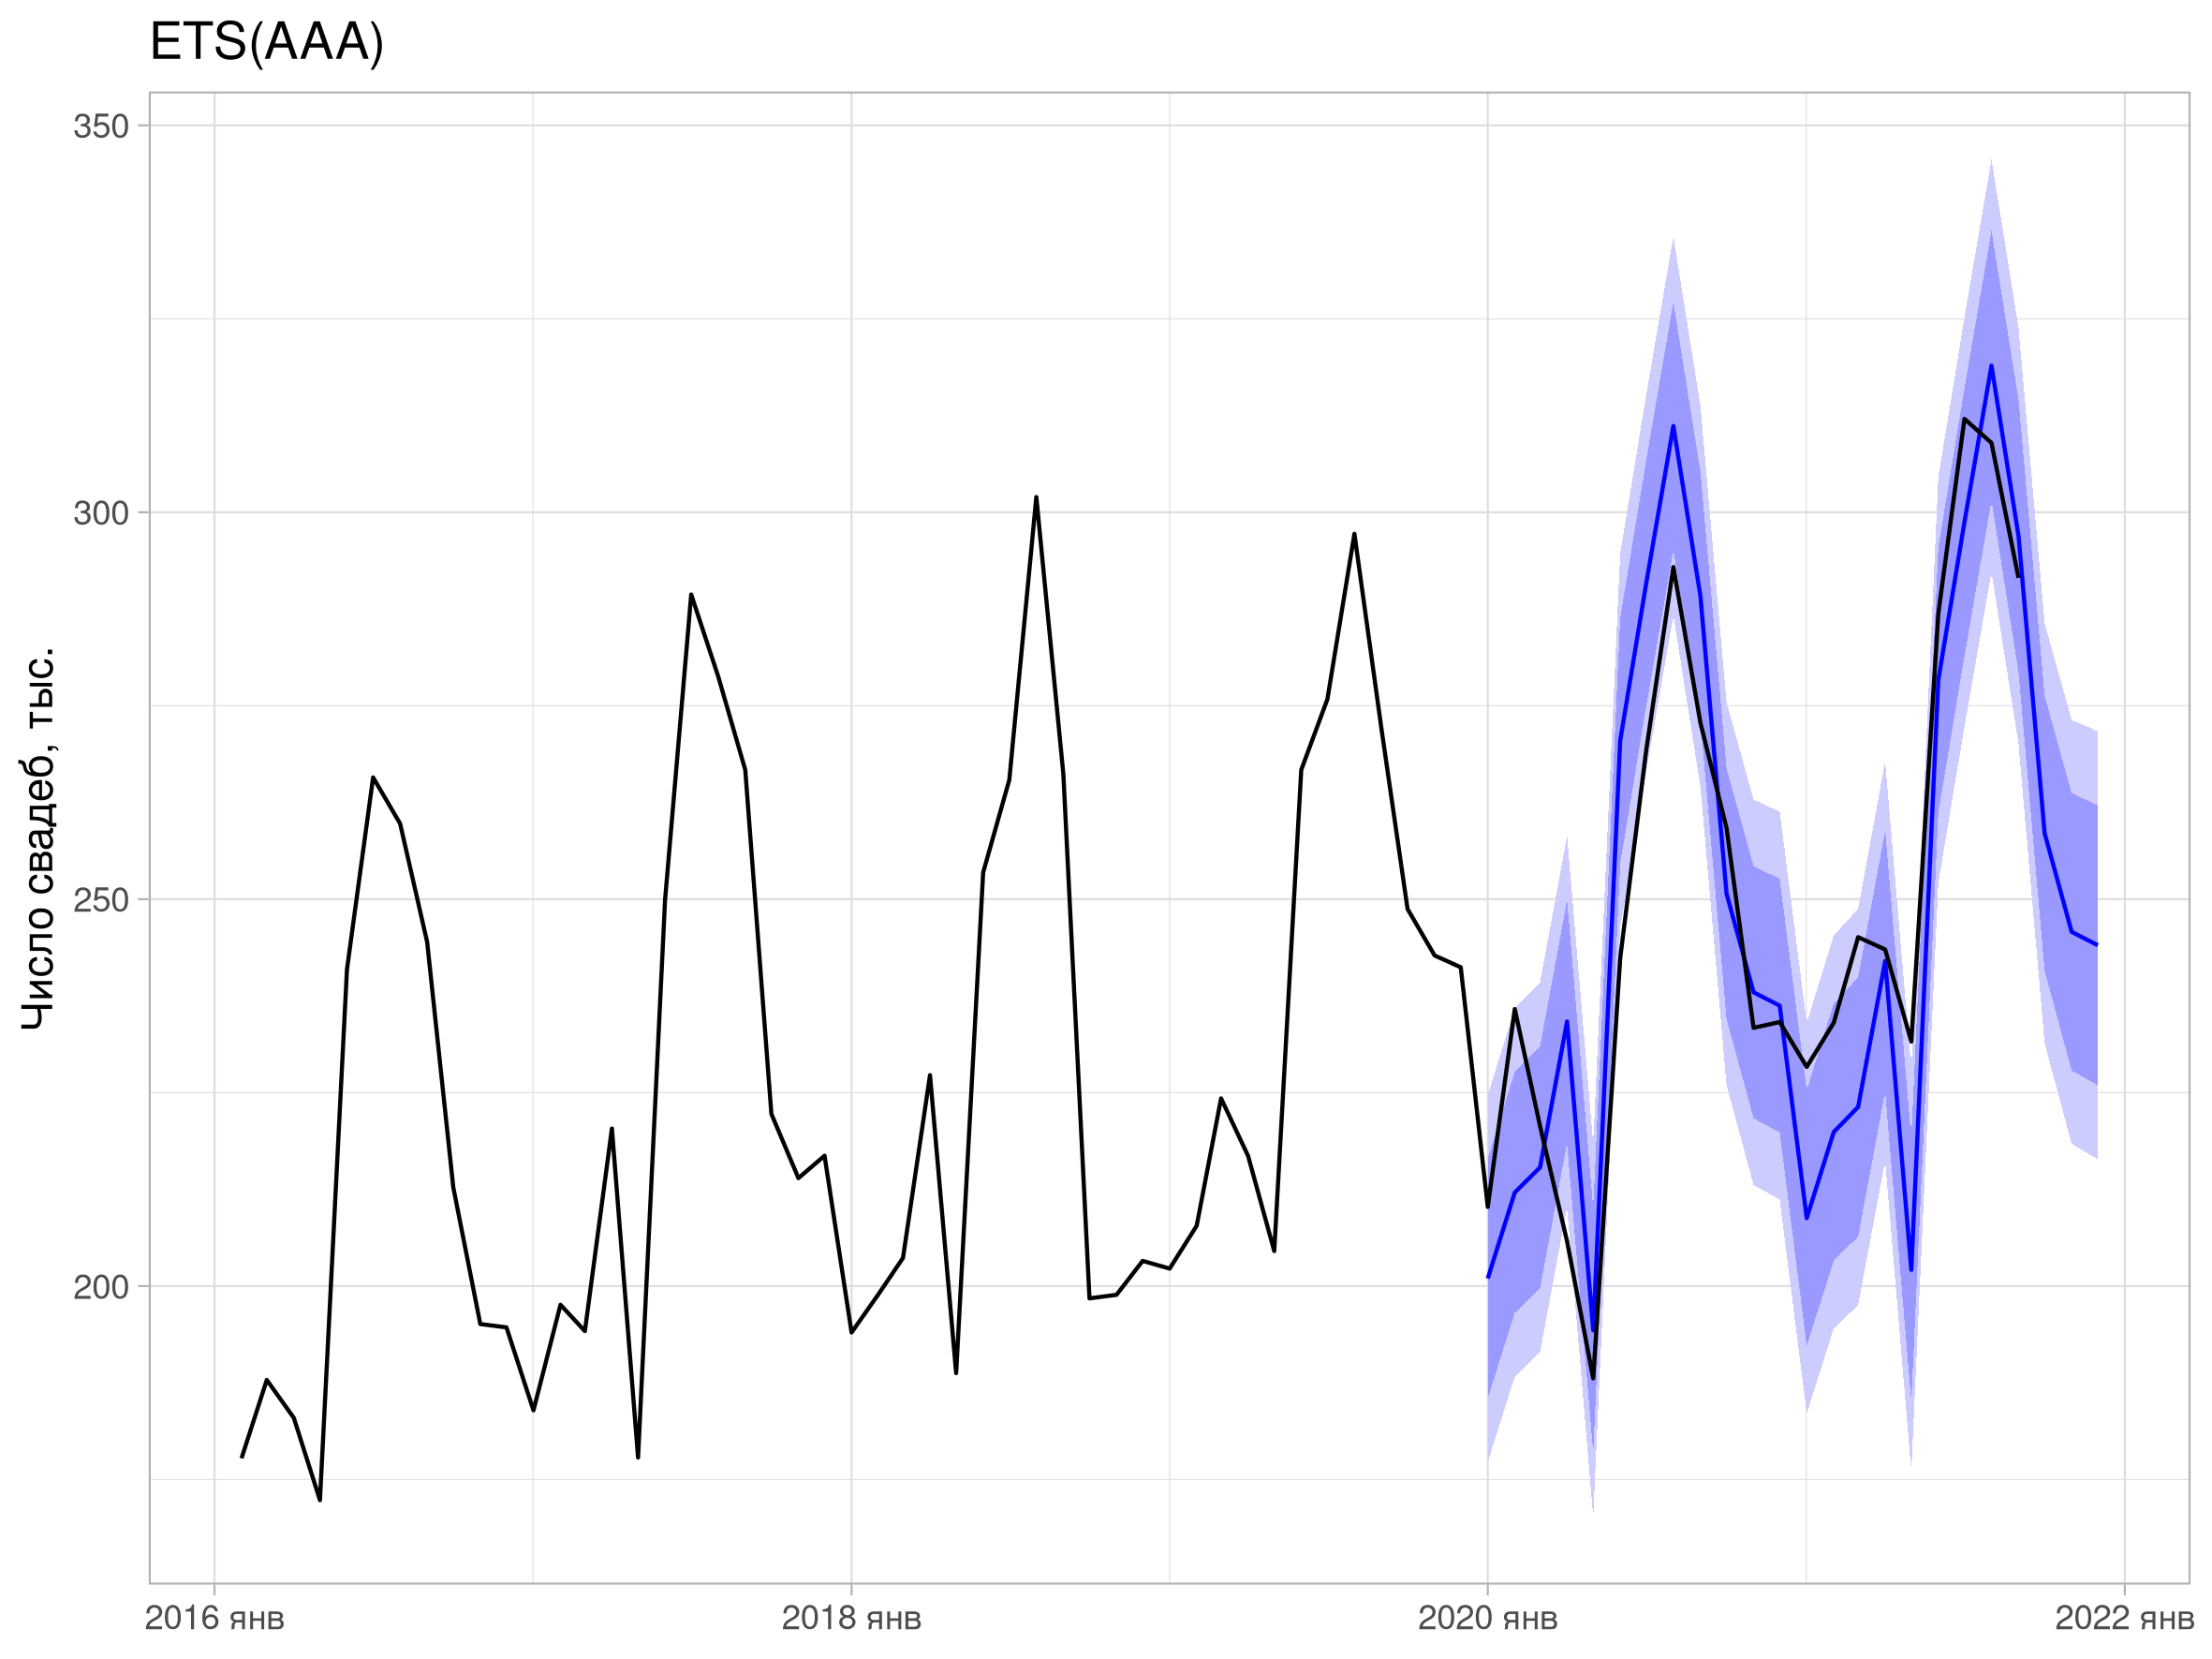
\includegraphics[width=\textwidth]{pictures/om_ts_02-076.png}


\end{frame}


\begin{frame}
  \frametitle{Прогноз на 1 шаг вперёд}

  \[
    \begin{cases}
     y_t = \ell_{t-1} + b_{t-1} + s_{t-12} + u_t; \\
    \ell_t = \ell_{t-1} + b_{t-1} + \alpha u_t, \text{ стартовое } \ell_0; \\
    u_t \sim \dN(0;\sigma^2) \text{ и независимы.} \\
    b_t = b_{t-1} + \beta u_t,\text{ стартовое } b_0; \\
    s_t = s_{t-12} + \gamma u_t
    \end{cases}
  \]
  \pause
\[
y_{T+1} = \ell_T + b_T + s_{T-11} + u_{T+1}  
\]
\pause
\[
  (y_{T+1} \mid \mathcal F_T) \sim \dN(\ell_T + b_T + s_{T-11}; \sigma^2)  
\]

\end{frame}


\begin{frame}
  \frametitle{Прогноз на 2 шага вперёд}

  \[
    \begin{cases}
        y_t = \ell_{t-1} + b_{t-1} + s_{t-12} + u_t; \\
       \ell_t = \ell_{t-1} + b_{t-1} + \alpha u_t, \text{ стартовое } \ell_0; \\
       u_t \sim \dN(0;\sigma^2) \text{ и независимы.} \\
       b_t = b_{t-1} + \beta u_t,\text{ стартовое } b_0; \\
       s_t = s_{t-12} + \gamma u_t
       \end{cases}
    \]
  \pause
  \begin{multline*}
    y_{T+2} = \ell_{T+1} + b_{T+1} + s_{T-10} + u_{T+2} = (\ell_T + b_T + \alpha u_{T+1}) +\\
    + (b_T + \beta u_{T+1}) + s_{T-10} + u_{T+2} 
  \end{multline*}
   \pause
  \[
  (y_{T+2} \mid \mathcal F_T) \sim \dN(\ell_T + 2b_T + s_{T-10}; \sigma^2((\alpha + \beta)^2 + 1))
  \]
  
\end{frame}


\begin{frame}
  \frametitle{Попутное разложение!}

  На выходе ETS(AAA):

  \alert{Оценки параметров}:  $\hat\alpha$, $\hat\beta$, $\hat\gamma$, $\hat\sigma^2$, $\hat\ell_0$, $\hat b_0$, 
  $\hat s_0$, $\hat s_{-1}$, \ldots, $\hat s_{-11}$.

  Ограничение: $\hat s_0 + \hat s_{-1} + \ldots + \hat s_{-11} = 0$.

  \pause 
  Оценённые \alert{значения составляющих}: $\hat \ell_t$, $\hat b_t$, $\hat s_t$.

  \pause 
  Автоматически получаем \alert{разложение}: $y_t = \hat \ell_t + \hat s_t + remainder_t$.

\end{frame}


\begin{frame}{ETS(AAA): итоги}

  \begin{itemize}[<+->]
    \item Ух, целых 17 параметров! 
    \item Наклон линии тренда и сезонность могут меняться.
    \item Автоматическое разложение на составляющие.
  \end{itemize}
\end{frame}





% !TEX root = ../om_ts_02.tex

\begin{frame} % название фрагмента

\videotitle{Много моделей}

\end{frame}



\begin{frame}{Много моделей: план}
  \begin{itemize}[<+->]
    \item Преобразование переменной. 
    \item Усреднение моделей. 
    \item Выбор с помощью кросс-валидации.
    \item Выбор с помощью AIC.
  \end{itemize}
\end{frame}

\begin{frame}{Преобразование переменной}
Помимо модели $y_t \sim ETS(AAA)$ можно оценить:

\pause
\alert{вторую модель} $\ln y_t \sim ETS(AAA)$ или \pause \alert{третью модель} $\sqrt{y_t} \sim ETS(AAA)$.

\pause 
Чтобы сравнивать прогнозы моделей, нужно работать в общем масштабе!

\pause
В \alert{зависимости от софта}: либо сами приводим к исходным единицам, либо это происходит автоматически. 
\end{frame}

\begin{frame}{Преобразование Бокса-Кокса}
Для $y_t$, чей размах колебаний растёт с ростом $y_t$, \alert{разумно попробовать} логарифм 
или преобразование Бокса-Кокса. 
\pause
Логарифм: $y_t \to \ln y_t$.

Преобразование Бокса-Кокса: $y_t \to bc_{\lambda}(y_t)$.

\pause

(\alert{Обобщённое}) преобразование Бокса-Кокса: 
\[
bc_{\lambda}(y_t) =
\begin{cases}
\ln y_t, \text{ если } \lambda = 0 \\
\sign(y_t) (\abs{y_t}^{\lambda} - 1)/\lambda, \text { если } \lambda \neq 0 \\
\end{cases}
\]

\end{frame}


\begin{frame}{Параметр лямбда}

    Как выбрать параметр $\lambda$ для перехода $y_t \to bc_{lambda}(y_t)$?

\[
bc_{\lambda}(y_t) =
\begin{cases}
\ln y_t, \text{ если } \lambda = 0 \\
\sign(y_t) (\abs{y_t}^{\lambda} - 1)/\lambda, \text { если } \lambda \neq 0 \\
\end{cases}
\]
\pause

\begin{itemize}[<+->]
    \item Некоторые модели содержат его внутри себя и сами подбирают $\lambda$.
    \item Можно подобрать $\lambda$ самостоятельно, чтобы стабилизировать амплитуду колебаний ряда. 
\end{itemize}
\end{frame}



\begin{frame}{Много моделей: итоги}

  \begin{itemize}[<+->]
    \item Сделать \alert{больше моделей}: преобразования переменной, усреднение моделей.
    \item Отобрать \alert{лучшую}: кросс-валидация, критерий AIC.
  \end{itemize}
\end{frame}



\end{document}
% !TEX root = ../om_metrics_14.tex

\begin{frame} % название фрагмента

\videotitle{Метод ближайших соседей}

\end{frame}



\begin{frame}{Метод ближайших соседей: план}
  \begin{itemize}[<+->]
    \item Использование соседей в задаче регрессии. 
    \item Кого считать соседом?
    \item Использование соседей в задаче классификации.
  \end{itemize}

\end{frame}


\begin{frame}{Метод $k$ ближайших соседей: регрессия}

\alert{Цель:} хотим спрогнозировать непрерывную величину $y$.
\pause


\alert{Не предполагаем} линейной зависимости $y$ от предикторов. 

\end{frame}

\begin{frame}

\begin{quotation}
  Скажи мне, кто твой друг, и я скажу, кто ты. 
\end{quotation}

\begin{minipage}[H]{0.9\linewidth}
  \begin{figure}
  \centering
    \caption{Мигель де Сервантес}
    \includegraphics[width=0.55\linewidth]{figures/Servantes.png}
  \end{figure}
\end{minipage}

\graylink{wikipedia.org}
\end{frame}


\begin{frame}{Ближайшие соседи}

Зависимая переменная: $y_i$.

Предикторы: $x_i = (a_i, b_i, c_i, \ldots)$.
\pause

Расстояние между двумя наблюдениями:

\[
d(x_1, x_2) = \sqrt{(a_1 - a_2)^2 + (b_1 - b_2)^2 + (c_1 - c_2)^2 + \ldots}  
\]
\pause

\begin{block}{Естественное определение}
  \alert{Ближайшими соседями} наблюдения $x$ называем те наблюдения, расстояние от него до которых наименьшее. 
\end{block}

\end{frame}

\begin{frame}{Прогнозирование}

\alert{Цель}: построить прогноз для $x = (a, b, c, \ldots)$.

\pause

Выбираем $k = 3$ ближайших соседей данного наблюдения. 

\pause 

Допустим это оказались наблюдения номер $5$, $42$ и $100$.

\pause

Считаем прогноз для вектора предикторов $x$ как среднее:
\[
\hat y = \frac{y_5 + y_{42} + y_{100}}{3}.
\]
\end{frame}

\begin{frame}{Треугольники — соседи квадрата}

\begin{center}
\includegraphics[scale=0.8]{figures/knn.png}
\end{center}

\end{frame}

\begin{frame}{Важность нормировки}

Расстояние \alert{чувствительно} к выбору масштаба.
\[
d(x_i, x_j) = \sqrt{(a_i - a_j)^2 + (b_i - b_j)^2 + (c_i - c_j)^2 + \ldots}  
\]

\pause

\alert{Важно} избавиться от единиц измерения!

\pause
Способ 1:
\[
a_i \to  \frac{a_i - \min(a)}{\max(a) - \min(a)}.
\]


\pause 

После преобразования все переменные лежат в отрезке $[0;1]$.

\pause

Данное масштабирование чувствительно к выбросам. 

\end{frame}


\begin{frame}{Избавиться от единиц измерения!}

  Способ 2:
  \[
  a_i \to \frac{a_i - \bar a}{\sqrt{\frac{\sum (a_i - \bar a)^2}{n - 1}}}.
  \]
  
  \pause 
  
  После преобразования каждая переменная имеет среднее равное нулю и 
  около 95\% её значений лежат в отрезке $[-2;2]$.
  
  \pause
  
  Данное масштабирование не учитывает выборочную корреляцию между переменными. 
  
\end{frame}



\begin{frame}{Избавиться от единиц измерения!}

  Способ 3: метрика Махаланобиса.
   \[
   x_i \to \left(\widehat{ \Var }(x_i)\right)^{-0.5} (x_i - \bar x)
   \]

\pause

Каждая новая переменная имеет среднее равное нулю и 
около $95\%$ её значений лежат в отрезке $[-2; 2]$.

\pause 
Новые переменные имеют нулевую выборочную корреляцию. 

\end{frame}


\begin{frame}{Как выбрать количество соседей?}

Основной способ: \alert{кросс-валидация}. 

\pause 
Для нескольких разных $k$, например, для $k \in \{1, 2, 3, 4, 5 \}$:

\begin{enumerate}[<+->]

\item Построим прогноз для каждого наблюдения, используя $k$ его ближайших соседей. 
\item Посчитаем сумму квадратов ошибок прогнозов
\[
  MSE_{k} = \frac{1}{n}\sum (y_i - \hat y_i^{cv})^2.
\]
\end{enumerate}
\pause
Выберем \alert{оптимальное} $k$.
\end{frame}



\begin{frame}{Задача классификации}


Что изменится, если $y$ — \alert{бинарная} переменная?  
\pause

Кратко: \alert{ничего}.

\pause
Зависимая переменная $y$ закодирована как $0$ и $1$, 
а $x_5$, $x_{42}$, $x_{100}$ — ближайшие наблюдения к $x$.


Считаем прогноз для вектора предикторов $x$ как среднее:
\[
\hat y = \frac{y_5 + y_{42} + y_{100}}{3}.
\]

\pause

Величина $\hat y$ — \alert{оценка вероятности} того, что $y = 1$.

\end{frame}

\begin{frame}{Метод $k$ ближайших соседей: итоги}

  \begin{itemize}[<+->]
    \item Предсказывает непрерывную или дискретную $y$.
    \item Не требует явного предположения \alert{о виде зависимости} от предикторов.
    \item Важно привести \alert{предикторы к общему масштабу}.
    \item \alert{Нет коэффициентов}, чтобы интерпретировать. 
    \item Можно комбинировать с другими методами.
  \end{itemize}
\end{frame}



% !TEX root = ../om_metrics_14.tex

\begin{frame} % название фрагмента

\videotitle{Метод ближайших соседей}

\end{frame}



\begin{frame}{Метод ближайших соседей: план}
  \begin{itemize}[<+->]
    \item Использование соседей в задаче регрессии. 
    \item Кого считать соседом?
    \item Использование соседей в задаче классификации.
  \end{itemize}

\end{frame}


\begin{frame}{Метод $k$ ближайших соседей: регрессия}

\alert{Цель:} хотим спрогнозировать непрерывную величину $y$.
\pause


\alert{Не предполагаем} линейной зависимости $y$ от предикторов. 

\end{frame}

\begin{frame}

\begin{quotation}
  Скажи мне, кто твой друг, и я скажу, кто ты. 
\end{quotation}

\begin{minipage}[H]{0.9\linewidth}
  \begin{figure}
  \centering
    \caption{Мигель де Сервантес}
    \includegraphics[width=0.55\linewidth]{figures/Servantes.png}
  \end{figure}
\end{minipage}

\graylink{wikipedia.org}
\end{frame}


\begin{frame}{Ближайшие соседи}

Зависимая переменная: $y_i$.

Предикторы: $x_i = (a_i, b_i, c_i, \ldots)$.
\pause

Расстояние между двумя наблюдениями:

\[
d(x_1, x_2) = \sqrt{(a_1 - a_2)^2 + (b_1 - b_2)^2 + (c_1 - c_2)^2 + \ldots}  
\]
\pause

\begin{block}{Естественное определение}
  \alert{Ближайшими соседями} наблюдения $x$ называем те наблюдения, расстояние от него до которых наименьшее. 
\end{block}

\end{frame}

\begin{frame}{Прогнозирование}

\alert{Цель}: построить прогноз для $x = (a, b, c, \ldots)$.

\pause

Выбираем $k = 3$ ближайших соседей данного наблюдения. 

\pause 

Допустим это оказались наблюдения номер $5$, $42$ и $100$.

\pause

Считаем прогноз для вектора предикторов $x$ как среднее:
\[
\hat y = \frac{y_5 + y_{42} + y_{100}}{3}.
\]
\end{frame}

\begin{frame}{Треугольники — соседи квадрата}

\begin{center}
\includegraphics[scale=0.8]{figures/knn.png}
\end{center}

\end{frame}

\begin{frame}{Важность нормировки}

Расстояние \alert{чувствительно} к выбору масштаба.
\[
d(x_i, x_j) = \sqrt{(a_i - a_j)^2 + (b_i - b_j)^2 + (c_i - c_j)^2 + \ldots}  
\]

\pause

\alert{Важно} избавиться от единиц измерения!

\pause
Способ 1:
\[
a_i \to  \frac{a_i - \min(a)}{\max(a) - \min(a)}.
\]


\pause 

После преобразования все переменные лежат в отрезке $[0;1]$.

\pause

Данное масштабирование чувствительно к выбросам. 

\end{frame}


\begin{frame}{Избавиться от единиц измерения!}

  Способ 2:
  \[
  a_i \to \frac{a_i - \bar a}{\sqrt{\frac{\sum (a_i - \bar a)^2}{n - 1}}}.
  \]
  
  \pause 
  
  После преобразования каждая переменная имеет среднее равное нулю и 
  около 95\% её значений лежат в отрезке $[-2;2]$.
  
  \pause
  
  Данное масштабирование не учитывает выборочную корреляцию между переменными. 
  
\end{frame}



\begin{frame}{Избавиться от единиц измерения!}

  Способ 3: метрика Махаланобиса.
   \[
   x_i \to \left(\widehat{ \Var }(x_i)\right)^{-0.5} (x_i - \bar x)
   \]

\pause

Каждая новая переменная имеет среднее равное нулю и 
около $95\%$ её значений лежат в отрезке $[-2; 2]$.

\pause 
Новые переменные имеют нулевую выборочную корреляцию. 

\end{frame}


\begin{frame}{Как выбрать количество соседей?}

Основной способ: \alert{кросс-валидация}. 

\pause 
Для нескольких разных $k$, например, для $k \in \{1, 2, 3, 4, 5 \}$:

\begin{enumerate}[<+->]

\item Построим прогноз для каждого наблюдения, используя $k$ его ближайших соседей. 
\item Посчитаем сумму квадратов ошибок прогнозов
\[
  MSE_{k} = \frac{1}{n}\sum (y_i - \hat y_i^{cv})^2.
\]
\end{enumerate}
\pause
Выберем \alert{оптимальное} $k$.
\end{frame}



\begin{frame}{Задача классификации}


Что изменится, если $y$ — \alert{бинарная} переменная?  
\pause

Кратко: \alert{ничего}.

\pause
Зависимая переменная $y$ закодирована как $0$ и $1$, 
а $x_5$, $x_{42}$, $x_{100}$ — ближайшие наблюдения к $x$.


Считаем прогноз для вектора предикторов $x$ как среднее:
\[
\hat y = \frac{y_5 + y_{42} + y_{100}}{3}.
\]

\pause

Величина $\hat y$ — \alert{оценка вероятности} того, что $y = 1$.

\end{frame}

\begin{frame}{Метод $k$ ближайших соседей: итоги}

  \begin{itemize}[<+->]
    \item Предсказывает непрерывную или дискретную $y$.
    \item Не требует явного предположения \alert{о виде зависимости} от предикторов.
    \item Важно привести \alert{предикторы к общему масштабу}.
    \item \alert{Нет коэффициентов}, чтобы интерпретировать. 
    \item Можно комбинировать с другими методами.
  \end{itemize}
\end{frame}



% !TEX root = ../om_metrics_14.tex

\begin{frame} % название фрагмента

\videotitle{Метод ближайших соседей}

\end{frame}



\begin{frame}{Метод ближайших соседей: план}
  \begin{itemize}[<+->]
    \item Использование соседей в задаче регрессии. 
    \item Кого считать соседом?
    \item Использование соседей в задаче классификации.
  \end{itemize}

\end{frame}


\begin{frame}{Метод $k$ ближайших соседей: регрессия}

\alert{Цель:} хотим спрогнозировать непрерывную величину $y$.
\pause


\alert{Не предполагаем} линейной зависимости $y$ от предикторов. 

\end{frame}

\begin{frame}

\begin{quotation}
  Скажи мне, кто твой друг, и я скажу, кто ты. 
\end{quotation}

\begin{minipage}[H]{0.9\linewidth}
  \begin{figure}
  \centering
    \caption{Мигель де Сервантес}
    \includegraphics[width=0.55\linewidth]{figures/Servantes.png}
  \end{figure}
\end{minipage}

\graylink{wikipedia.org}
\end{frame}


\begin{frame}{Ближайшие соседи}

Зависимая переменная: $y_i$.

Предикторы: $x_i = (a_i, b_i, c_i, \ldots)$.
\pause

Расстояние между двумя наблюдениями:

\[
d(x_1, x_2) = \sqrt{(a_1 - a_2)^2 + (b_1 - b_2)^2 + (c_1 - c_2)^2 + \ldots}  
\]
\pause

\begin{block}{Естественное определение}
  \alert{Ближайшими соседями} наблюдения $x$ называем те наблюдения, расстояние от него до которых наименьшее. 
\end{block}

\end{frame}

\begin{frame}{Прогнозирование}

\alert{Цель}: построить прогноз для $x = (a, b, c, \ldots)$.

\pause

Выбираем $k = 3$ ближайших соседей данного наблюдения. 

\pause 

Допустим это оказались наблюдения номер $5$, $42$ и $100$.

\pause

Считаем прогноз для вектора предикторов $x$ как среднее:
\[
\hat y = \frac{y_5 + y_{42} + y_{100}}{3}.
\]
\end{frame}

\begin{frame}{Треугольники — соседи квадрата}

\begin{center}
\includegraphics[scale=0.8]{figures/knn.png}
\end{center}

\end{frame}

\begin{frame}{Важность нормировки}

Расстояние \alert{чувствительно} к выбору масштаба.
\[
d(x_i, x_j) = \sqrt{(a_i - a_j)^2 + (b_i - b_j)^2 + (c_i - c_j)^2 + \ldots}  
\]

\pause

\alert{Важно} избавиться от единиц измерения!

\pause
Способ 1:
\[
a_i \to  \frac{a_i - \min(a)}{\max(a) - \min(a)}.
\]


\pause 

После преобразования все переменные лежат в отрезке $[0;1]$.

\pause

Данное масштабирование чувствительно к выбросам. 

\end{frame}


\begin{frame}{Избавиться от единиц измерения!}

  Способ 2:
  \[
  a_i \to \frac{a_i - \bar a}{\sqrt{\frac{\sum (a_i - \bar a)^2}{n - 1}}}.
  \]
  
  \pause 
  
  После преобразования каждая переменная имеет среднее равное нулю и 
  около 95\% её значений лежат в отрезке $[-2;2]$.
  
  \pause
  
  Данное масштабирование не учитывает выборочную корреляцию между переменными. 
  
\end{frame}



\begin{frame}{Избавиться от единиц измерения!}

  Способ 3: метрика Махаланобиса.
   \[
   x_i \to \left(\widehat{ \Var }(x_i)\right)^{-0.5} (x_i - \bar x)
   \]

\pause

Каждая новая переменная имеет среднее равное нулю и 
около $95\%$ её значений лежат в отрезке $[-2; 2]$.

\pause 
Новые переменные имеют нулевую выборочную корреляцию. 

\end{frame}


\begin{frame}{Как выбрать количество соседей?}

Основной способ: \alert{кросс-валидация}. 

\pause 
Для нескольких разных $k$, например, для $k \in \{1, 2, 3, 4, 5 \}$:

\begin{enumerate}[<+->]

\item Построим прогноз для каждого наблюдения, используя $k$ его ближайших соседей. 
\item Посчитаем сумму квадратов ошибок прогнозов
\[
  MSE_{k} = \frac{1}{n}\sum (y_i - \hat y_i^{cv})^2.
\]
\end{enumerate}
\pause
Выберем \alert{оптимальное} $k$.
\end{frame}



\begin{frame}{Задача классификации}


Что изменится, если $y$ — \alert{бинарная} переменная?  
\pause

Кратко: \alert{ничего}.

\pause
Зависимая переменная $y$ закодирована как $0$ и $1$, 
а $x_5$, $x_{42}$, $x_{100}$ — ближайшие наблюдения к $x$.


Считаем прогноз для вектора предикторов $x$ как среднее:
\[
\hat y = \frac{y_5 + y_{42} + y_{100}}{3}.
\]

\pause

Величина $\hat y$ — \alert{оценка вероятности} того, что $y = 1$.

\end{frame}

\begin{frame}{Метод $k$ ближайших соседей: итоги}

  \begin{itemize}[<+->]
    \item Предсказывает непрерывную или дискретную $y$.
    \item Не требует явного предположения \alert{о виде зависимости} от предикторов.
    \item Важно привести \alert{предикторы к общему масштабу}.
    \item \alert{Нет коэффициентов}, чтобы интерпретировать. 
    \item Можно комбинировать с другими методами.
  \end{itemize}
\end{frame}



\end{document}
